%!TEX root = ../Main.tex

\section{Methodology and Data}

\subsection{Data and Calculation of Input Factors}
The data used in this study are from several sources. The realized variance of the S\&P 500 .. . Then write about what data adjustments were made, including the ones already done with oxford realized library.

Also \citeauthor{andersen2003} point out the advantage of using high-frequency returns is not only that they help predicting again high-frequency returns, but also that they contain information for longer horizons, such as monthly or quarterly. 
Graphics

VIX is the daily implied volatility index, calculated from the annualized volatility as VIX/$\sqrt{252}$ as in \textcite{blair2000} and \textcite{whaley2008}. \\

For an analysis of the historic values of the VIX, see \textcite{whaley2008} (chapter: historix, normal range). 


\begin{figure}[!htbp]
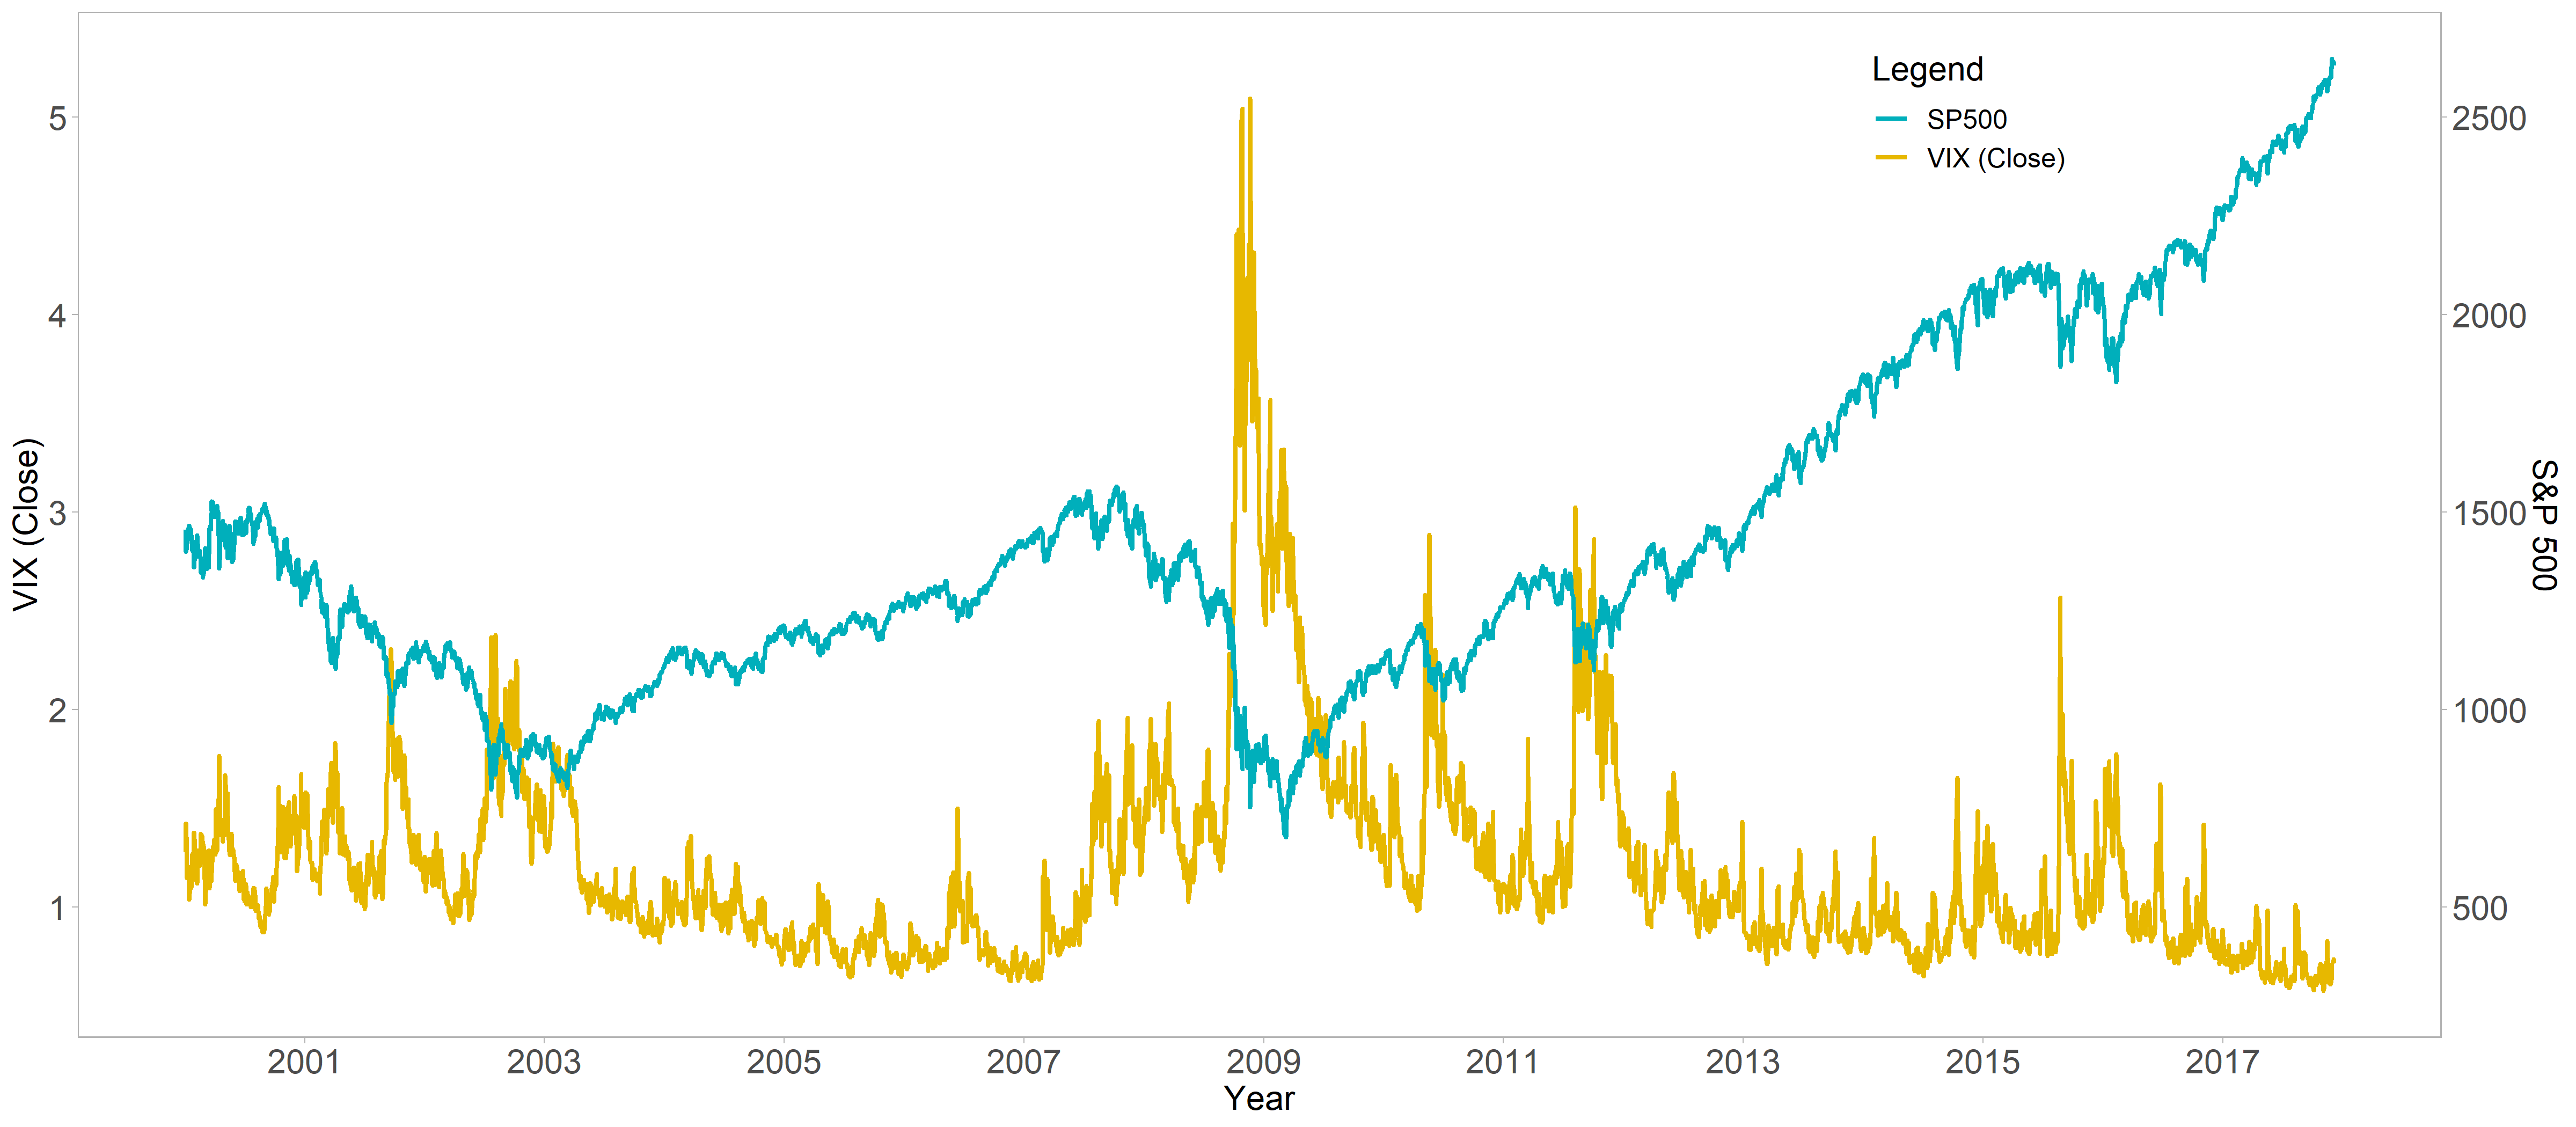
\includegraphics[width=16cm, height=8cm]{pictures/SPandViX.png}
\end{figure}

\begin{figure}[!htbp]
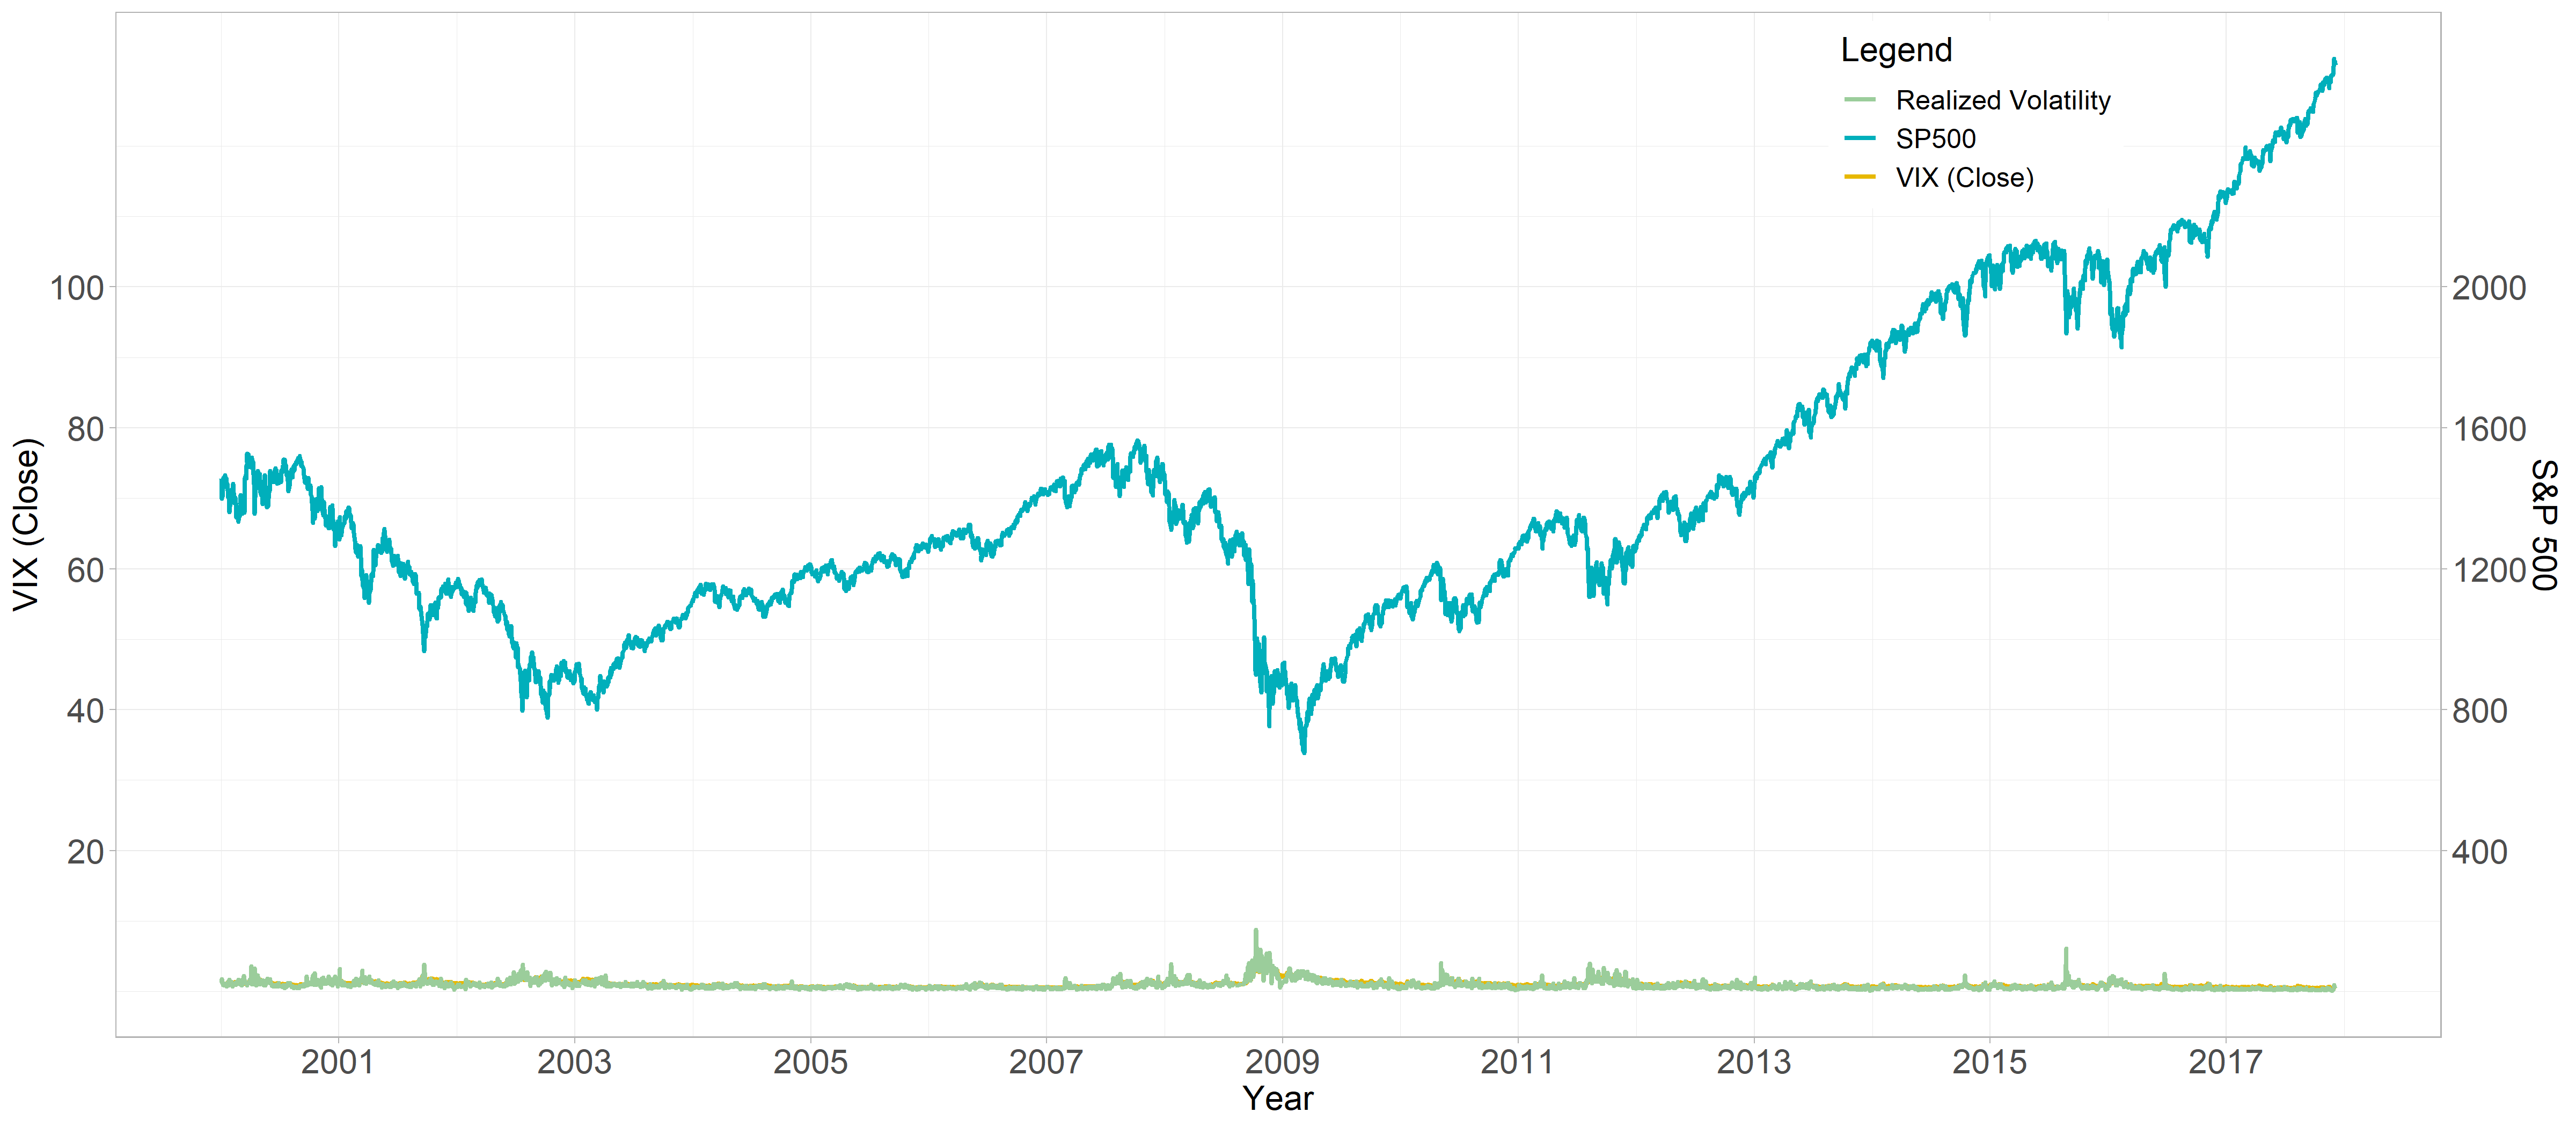
\includegraphics[width=16cm, height=8cm]{pictures/SPandVolandViX.png}
\end{figure}

Measure for daily return variability should be realized volatility, as \citeauthor{andersen2001} suggest, that under suitable conditions it provides an unbiased estimator of the return volatility. 


\begin{itemize}\itemsep0pt
\item S\&P 500 index data on daily basis
\item sampling period: 2000 - 2018
\item realized volatility: daily realized volatility of S\&P 500, calculated using 5 minute returns, retrieved from \citeauthor{heber2009}
\item model-free implied volatility: VIX index data
\item historic volatility: lagged realized volatility, for HAR-RV model use the average over the time period used to forecast
\end{itemize}


\subsection{Methodology: Linear Regression and HAR-RV model}
Consistent with prior research, for example \textcite{jiang2003}, \textcite{canina1993} or \textcite{christensen1998}, both univariate and encompassing regression analysis is used to analyse the information content of volatility measures. In the univariate regression, the realized volatility is only regressed on the historic data. For comparison, realized volatility is regressed on both historic data and the VIX in the encompassing regression analysis. Thus the encompassing regression analysis gives information about the relative importance of the volatility measures, and whether the VIX as one of them subsumes the information from the historic volatility. The two regressions are then given by:
\begin{align}
RV_{t+1d} = c + \beta^{d} RV^{d}_{t} + \beta^{w} RV^{w}_{t} + \beta^{m} RV^{m}_{t}  \\
RV_{t+1d} = c + \beta^{d} RV^{d}_{t} + \beta^{w} RV^{w}_{t} + \beta^{m} RV^{m}_{t} + \beta^{VIX} VIX
\end{align}
with .. (explain variables again?). In alignment with \textcite{corsi2009}, the Newey-West covariance correction is used, to account for the possible presence of serial correlation in the data, as serial correlation causes both the Gauss-Markow and Classical linear model assumptions to fail. 


\subsection{Limitations}
As volatility is stochastic, the ex-ante estimation will not equal the return volatility, as it is a measurement over an aggregated discrete time period \parencite{andersen2001}.
The VIX might be flawed, as \textcite{jiang2007} showed.
